%\documentclass[twoside,a4paper,11pt]{book}
\documentclass[a4paper,11pt,oneside]{book}

%----------------------------------------------------------------------------------------
%	README!
%   Welcome. It's worth having a read through this file
%   to set up the broad parameters, such as the name of
%   the degree, the school/department, the type of work
%   (dissertation/Final Year Project/report, etc. as well
%   as your own details.
%----------------------------------------------------------------------------------------

%----------------------------------------------------------------------------------------
%	COVER PAGE
%   The cover page is laid out in title/title.tex. You can choose a colour
%   or black and white logo
%----------------------------------------------------------------------------------------

%----------------------------------------------------------------------------------------
%	THESIS INFORMATION
%   Put title, author name, supervisor name, degree, type of work, school, department in here
%   It will be used for the title page and for the embedded PDF information
%----------------------------------------------------------------------------------------

\newcommand{\thesistitle}{Evaluation of Proximal Policy Optimisation in Continual Reinforcement Learning} % Your thesis title, this is used in the title and abstract
\newcommand{\CSE}{M.Sc. Computer Science (Data Science)} % Replace with your degree name, this is used in the title page and abstract
\newcommand{\typeofthesis}{dissertation} % dissertation, Final Year Project, report, etc.
\newcommand{\authorname}{Kim Nia Nolle} % Your name, this is used in the title page and PDF stuff
%% Do not put your Student ID in the document, as TCD will not publish
%% documents that contain both your name and your Student ID.
\newcommand{\supervisor}{Prof. Vinny Cahill} % replace with the name of your supervisor
\newcommand{\cosupervisor}{Wenlong Wang} % replace with the name of your co-supervisor if you have one
\newcommand{\keywords}{this, that, more} % Replace with keywords for your thesis
\newcommand{\school}{\href{https://www.tcd.ie/scss/}{School of Computer Science and Statistics}} % Your school's name and URL, this is used in the title page
%Edited by HS for engineering

%% Comment out the next line if you don't want a department to appear
%\newcommand{\department}{\href{http://researchgroup.university.com}{Department Name}} % Your research group's name and URL, this is used in the title page


%% Language and font encodings
\usepackage[T1]{fontenc} 
\usepackage[utf8]{inputenc}
\usepackage[english]{babel}

%% Bibliographical stuff
%\usepackage[]{cite}
%% Document size
% include showframe as an option if you want to see the boxes
\usepackage[a4paper,top=2.54cm,bottom=2.54cm,left=3cm,right=3cm,headheight=16pt]{geometry}
\setlength{\marginparwidth}{2cm}
%% Useful packages
\usepackage{amssymb}
\usepackage{amsmath}
\usepackage[autostyle=true]{csquotes} % Required to generate language-dependent quotes in the bibliography
\usepackage[pdftex]{graphicx}
\usepackage[colorinlistoftodos]{todonotes}
\usepackage[colorlinks=true, allcolors=black]{hyperref}
\usepackage{hyperxmp}
\usepackage{caption} % if no caption, no colon
\usepackage{sfmath} %use sans-serif in the maths sections too
\usepackage[parfill]{parskip}    % Begin paragraphs with an empty line rather than an indent
\usepackage{setspace} % to permit one-and-a-half or double spacing
\usepackage{enumerate} % fancy enumerations like (i) (ii) or (a) (b) and suchlike
\usepackage{booktabs} % To thicken table lines
\usepackage{fancyhdr}
\usepackage{xcolor} % to get TCD colour on headings
\numberwithin{equation}{chapter} %HS edit for (chapter.equation)
\pagestyle{plain} % Embrace simplicity!
%\usepackage{hyperref}
\usepackage{float}

\usepackage[acronym,nomain,automake]{glossaries}
\makeglossaries

\definecolor{tcd_blue}{RGB}{5, 105, 185}

%% It's personal taste but...
%% Uncomment the following block if you want your name and ID at the top of
%% (almost) every page.
%\fancyhf{} % sets both header and footer to nothing
%\renewcommand{\headrulewidth}{0pt}
%\cfoot{\thepage}
%\ifdefined\authorid
%\chead{\it \authorname\ (\authorid)}
%\else
%\chead{\it \authorname}
%\fi
%% End of block

%% It is good practise to make your font sans-serif to improve the accessibility of your document.  Comment out the following line to disable it (but you really should not)
\renewcommand{\familydefault}{\sfdefault} %use the sans-serif font as default

%% If you insist on not using sans-serif (please don't), consider using Palatino instead of the LaTeX standard
%\usepackage{mathpazo} % Use the Palatino font by default if you prefer it to Computer Modern


%% Format Chapter headings appropriately
\usepackage{titlesec}
\titleformat{\chapter}[hang]{\normalfont\Huge\bfseries\color{tcd_blue}}{\thechapter.}{0.5em}{}{}
\titlespacing{\chapter}
{0pt} %left of the label + title
{*0} % vertical space before the title
{*6.5} % idem after title (in ex units + glue)

\title{\thesistitle}
\author{\authorname}


\hypersetup{
   pdftitle=\thesistitle, % Set the PDF's title to your title
   pdfauthor=\authorname, % Set the PDF's author to your name
   pdfkeywords=\keywords, % Set the PDF's keywords to your keywords
   pdfsubject=\CSE, % Set the PDF's keywords to your keywords
   pdfinfo={
     pdfsupervisor=\supervisor, % Set the PDF's supervisor to your supervisor
     pdfcosupervisor=\cosupervisor, % Set the PDF's cosupervisor to your cosupervisor if using
   }
}

%% Imports the biblatex package
\usepackage[
backend=biber,
style=authoryear,
%sorting=none
]{biblatex}

%% Imports the bibliography file "bibFile.bib" containing the sources of the citations
\bibliography{bibs}

%\frontmatter


\begin{document}
\date{August 31, 2024}
%\dominitoc[n]               % generate minitocs for every chapter
\pagenumbering{Roman}       % set page numbers to roman style

\begin{titlepage}
\center % Center everything on the page

%% All the text parameters should be taken from the start of the main.tex file.
%% You should only alter stuff here if you want to change the layout

%----------------------------------------------------------------------------------------
%	LOGO SECTION
%----------------------------------------------------------------------------------------
%% Choose one of the following -- a colour or black-and-white logo


\includegraphics{title/Trinity_RGB_transparent_main.png}\\[1cm] 
%
\includegraphics[width=12cm]{title/black-stacked-trinity.jpg}\\[1cm] 

\Large \school\\[1.5cm] % Minor heading such as course title
\ifdefined\department
\large \department\\[1.5cm] % Minor heading such as course title
\fi

%----------------------------------------------------------------------------------------
%	TITLE SECTION
%----------------------------------------------------------------------------------------
\makeatletter
{ \huge \bfseries \thesistitle}\\[1.5cm] % Title of your document
 

%----------------------------------------------------------------------------------------
%	AUTHOR SECTION
%----------------------------------------------------------------------------------------

\ifdefined\authorid
\authorname\\ % Your name
\authorid\\[2cm] % Your Student ID
\else
\authorname\\[2cm] % Your name
\fi

%----------------------------------------------------------------------------------------
%	Supervisor SECTION
%----------------------------------------------------------------------------------------

Supervisor: \supervisor\\[0.5cm] % Their name
\ifdefined\cosupervisor
Co-Supervisor: \cosupervisor\\[2cm] % Their name
\fi


%----------------------------------------------------------------------------------------
%	DATE SECTION
%----------------------------------------------------------------------------------------

{\large \@date}\\[2cm] % Date, change the \today to a set date if you want to be precise

 
%----------------------------------------------------------------------------------------
%	TYPE OF THESIS SECTION
%----------------------------------------------------------------------------------------
\vfill
 A \typeofthesis\ submitted in partial fulfilment\\of the requirements for the degree of \\
\CSE

\vfill % Fill the rest of the page with whitespace

\end{titlepage}             % title page with subject and print date
\linespread{1.2}            % line spacing factor -> causes trouble with minitoc!
%\noitemsep % conflicts with enumitem
%\setlist[itemize]{noitemsep}
%\setlist[enumerate]{noitemsep}
%\setlist[description]{noitemsep}

\setcounter{page}{1}   % modify start value (for book-version only)
\chapter*{Declaration}
\label{sec:Declaration} %
\addcontentsline{toc}{section}{Declaration}

%\vspace{1cm}
I hereby declare that this \typeofthesis\ is entirely my own work and that it has not been submitted as an exercise for a degree at this or any other university.

\vspace{0.5cm}
I have read and I understand the plagiarism provisions in the General Regulations of the University Calendar for the current year, found at \url{http://www.tcd.ie/calendar}.
\vspace{0.5cm}

I have completed the Online Tutorial on avoiding plagiarism `Ready Steady Write', located at \url{http://tcd-ie.libguides.com/plagiarism/ready-steady-write}.
\vspace{0.5cm}

I consent / do not consent to the examiner retaining a copy of the thesis beyond the examining period, should they so wish (EU GDPR May 2018).
\vspace{0.5cm}

I agree that this thesis will not be publicly available, but will be available to TCD staff and students in the University’s open access institutional repository on the Trinity domain only, subject to Irish Copyright Legislation and Trinity College Library conditions of use and acknowledgement.  \textbf{Please consult with your supervisor on this last item before agreeing, and delete if you do not consent}
\vspace{3cm}

Signed:~\rule{5cm}{0.3pt}\hfill Date:~\rule{5cm}{0.3pt}
%
\chapter*{Abstract}
\label{sec:Abstract}%
% add this page manually to the table of contents with ROMAN letters
\addcontentsline{toc}{section}{Abstract}
%

Summary of the dissertation 

\vspace{1cm}

\textbf{Keywords:} \keywords



%
\chapter*{Acknowledgements}
\label{sec:Ack}%
% add this page manually to the table of contents with ROMAN letters
\addcontentsline{toc}{section}{Acknowledgements}
%


Thank you to ...

%\gls{} : This command prints the term in lowercase characters.
%\Gls{} : This is similar to \gls{ } command. The only difference is it will print the first character in the uppercase.
%\glspl{} : This command is similar to \gls{ }. The only difference is that it will convert the term into its plural form.
%\Glspl{} : This command is similar to \Gls{ } command, with the difference that it will convert the term in its plural also.


%\newacronym{}{}{}
%\newacronym[first=CSV]{csv}{CSV}{\textit{Comma-separated values}}

\newacronym{dqn}{DQN}{Deep Q-Learning}
\newacronym{sgd}{SGD}{Stochastic Gradient Descent}
\newacronym{iid}{i.i.d.}{independent and identically distributed}
\newacronym{rl}{RL}{Reinforcement Learning}
\newacronym{cl}{CL}{Continual Learning}
\newacronym{mdp}{MDP}{Markov Decision Process}
\newacronym[plural=POMDP,firstplural=Partially Observable Markov Decision Processes (POMDP)]{pomdp}{POMDP}{Partially Observable Markov Decision Process}
%*************************************************
%
%       Lists
%       C.Koch
%       Created 02.02.2001
%
%*************************************************


\tableofcontents
%\addcontentsline{toc}{section}{List of Figures}%
\listoffigures %
%\addcontentsline{toc}{section}{List of Tables}%
\listoftables
%
%\lstlistoflistings
%\listofcodes

\printglossaries
%\printglossary[type=\acronymtype, nonumberlist]
%\printnoidxglossary[type=\acronymtype,title=Acronyms]




\cleardoublepage
%\linespread{0.6} %  default line spread

%\linespread{1.2} % current line spread
%
\newpage


\cleardoublepage            % for correct page numbering / margin
\pagenumbering{arabic}      % reset page numbers to arabic style


% \chapter*{Abstract}
% A short summary of the problem investigated, the approach taken and the key findings. This should not be more that around 400 words.


% This must be on a separate page.

% \chapter*{Lay Abstract}
% Similar to the actual abstract in terms of the information, but written for a non-specialist. So no jargon, no acronyms. Explain to a member of the general public what this project entailed. Should be no longer than the actual abstract.


%This must be on a separate page.

%\newpage
\onehalfspacing%\raggedright %\raggedright turns off justification and hyphenation

% \section*{\Huge\textcolor{tcd_blue}{Acknowledgements}}
% Thanks Everyone!

% You should acknowledge any help that you have received (for example from technical staff), or input provided by, for example, a company.
% \tableofcontents
% \listoffigures
% \listoftables
% \newpage
% \section*{\Huge\textcolor{tcd_blue}{Nomenclature}}
% \begin{tabular}{lp{9cm}l}
% A&Area of the wing&$m^{2}$\\
% B\\
% C& Roman letters first, with capitals\ldots\\
% a&then lower case.\\
% b\\
% c\\
% $\Gamma$&Followed by Greek capitals\ldots\\
% $\alpha$&then lower case greek symbols.\\
% $\beta$\\
% $\epsilon$\\
% TLA&Finally, three letter acronyms and other abbreviations arranged alphabetically\\
% \end{tabular}
% \vspace{2cm}

% If a parameter has a typical unit that is used throughout your report, then it should be included here on the right hand side.

% If you have a very mathematical report, then you may wish to divide the nomenclature list into functions and variables, and then sub- and super-scripts.

% If you have a large number of acronyms, check out \href{https://www.overleaf.com/learn/latex/Glossaries} to make that more robust.

% Note that Roman mathematical symbols are typically in a serif font in italics.
\glsresetall
\chapter{Introduction}

Despite rising costs and the climate-crisis, driving continues to be one of the most popular modes of transportation. One major problem with the high traffic demands is traffic congestion. The \cite{TomTom_2023} Traffic Index has shown that a majority of global cities have seen a rise in travel times in 2023 compared to the previous year, especially during peak hours. Not only does traffic congestion lead to an increase in travel times, but it is also associated with increased greenhouse gas emissions and air pollution \parencite{DoT_2023}, which in turn are linked to health risks such as cardiovascular and respiratory diseases \parencite{WHO_2022}. 

In order to curb these issues, effective traffic management is needed. This can be achieved for example by using traffic lights to control the flow of traffic. However, inefficient traffic light cycles can worsen congestion, for example through cross-blocking (when the downstream lane is full so that a vehicle cannot cross the intersection) or green-idling (when a green signal is active even though there are no vehicles crossing in that direction) \parencite{Rasheed_2020}. 

One promising approach to dynamically optimising traffic light cycles is \gls{rl} because no prior assumptions about the systems are required \parencite{Liu_2023}. Most research in utilising \gls{rl} for traffic light control is based on \gls{dqn} \parencite{Rasheed_2020}, which uses \gls{sgd} for optimisation \parencite{Mnih_2015}. \gls{sgd} and \gls{sgd}-based algorithms assume stationary \gls{iid} data distributions \parencite{Khetarpal_2022}. However, the environment in traffic control can be considered non-stationary because, for example, the distribution of traffic demand varies over time (higher demand during rush hours etc.). Blindly applying these approaches in non-stationary settings can lead to biased optimisations and catastrophic forgetting \parencite{Khetarpal_2022}. It is therefore important to approach traffic control with \gls{cl}, an \gls{rl} paradigm that takes non-stationarity into account.

CL agents need to be able to adapt quickly to changes in the environment \parencite{Khetarpal_2022}. \gls{dqn} is an off-policy algorithm \parencite{Mnih_2015}, which have more variance and converge slower than on-policy methods \parencite{SuttonBarto_2018}. An on-policy algorithm such as PPO \parencite{Schulman_2017} may therefore be more suited for traffic control problems.


\section{Research Objectives}
Research Question

Can Proximal Policy Optimization (PPO) and experience replay be combined for effective learning in a continual learning environment?

Understand behaviour of PPO agents in continual learning environments

Investigate whether experience replay can be used to mitigate problems such as catastrophic forgetting

Propose and evaluate possible improvements

\section{Methodology}
Introduce how these objectives will be achieved

\section{Dissertation Structure}
Overview of diffrerent chapters
\chapter{State of the Art}

This chapter presents background knowledge on \gls{rl} and \gls{cl}. Related works on \gls{cl} approaches and the use of \gls{rl} in urban traffic control are also reviewed.

\section{Reinforcement Learning}

Reinforcement Learning (\gls{rl}) is a machine learning paradigm in which a so-called agent develops a behaviour by learning how to maximise a numerical reward through interacting with its environment \parencite{SuttonBarto_2018}. This differs from both supervised and unsupervised learning \parencite{Yang_2019}. Supervised learning uses labelled data to model the data. Unsupervised learning uses unlabelled data to identify structures in the data. In contrast to this, \gls{rl} aims to maximise reward rather than learn patterns and structures in data.

The interactions between an agent and its environment can be formalised as a \gls{mdp} \parencite{SuttonBarto_2018}. An \gls{mdp} is defined by a state space $\mathcal{S}$, an action space $\mathcal{A}$, a set of rewards $\mathcal{R}$ and a transition probability function $p$. The diagram in \autoref{fig:interaction-MDP} shows the process of the interaction. At each time step $t$, the agent selects an action $A_t\in \mathcal{A}$ based on the current state $S_t \in \mathcal{S}$. According to the dynamics of the environment, represented by the $p$-function, the environment emits a reward $R_{t+1} \in \mathcal{R}$ and the next state $S_{t+1}$ in response.
The general definition of the $p$-function is given by \autoref{equ:p-func}.

\begin{equation}
\label{equ:p-func}
p(s', r|s, a)=Pr\lbrace S_{t+1}=s', R_{t+1}=r|S_t=s, A_t=a\rbrace
\end{equation}


\begin{figure}[H]
\centering
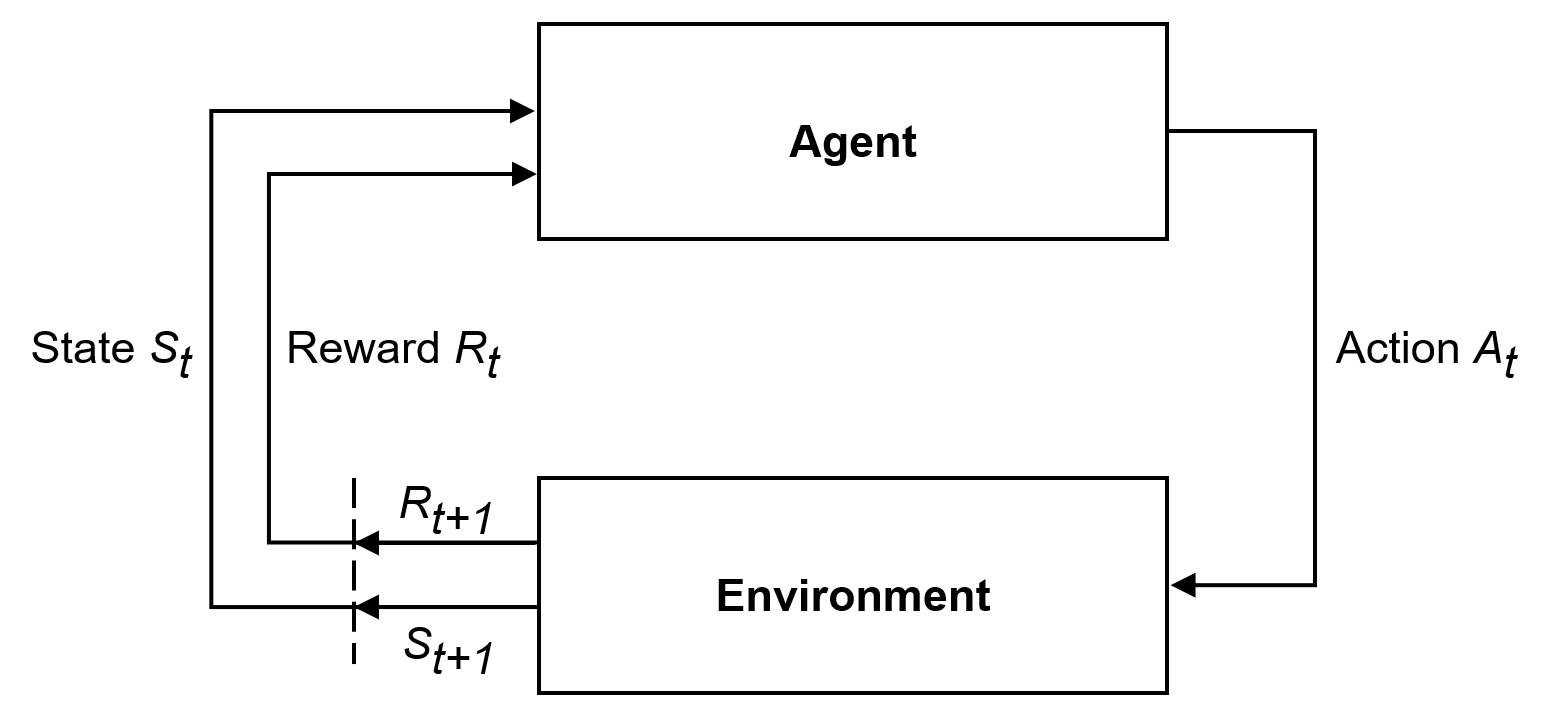
\includegraphics[height=5cm]{img/agent-env_MDP.png}
\caption{MDP framework (based on \textcite{SuttonBarto_2018})}
\label{fig:interaction-MDP}
\end{figure}

This framework can be generalised further (as shown in \autoref{fig:interaction-POMDP}) to also describe Partially Observable MDPs (\glsunset{pomdp}\gls{pomdp}) \parencite{silver2015}. \glspl{pomdp} are cases in which the agent is unable to fully observe the state of the environment.
In this framework, $S_t^e$ denotes the environment state. The observation $O_t$ is the information about the environment state that is emitted to the agent. In a \gls{pomdp}, the agent's internal representation of the state $S^a_t$ differs from $S_t^e$ and is constructed for example as a function of the previous state $S^a_{t-1}$ and the observation $O_t$. An \gls{mdp} is a special case where $O_t=S_t^e=S^a_t$.

\begin{figure}[H]
\centering
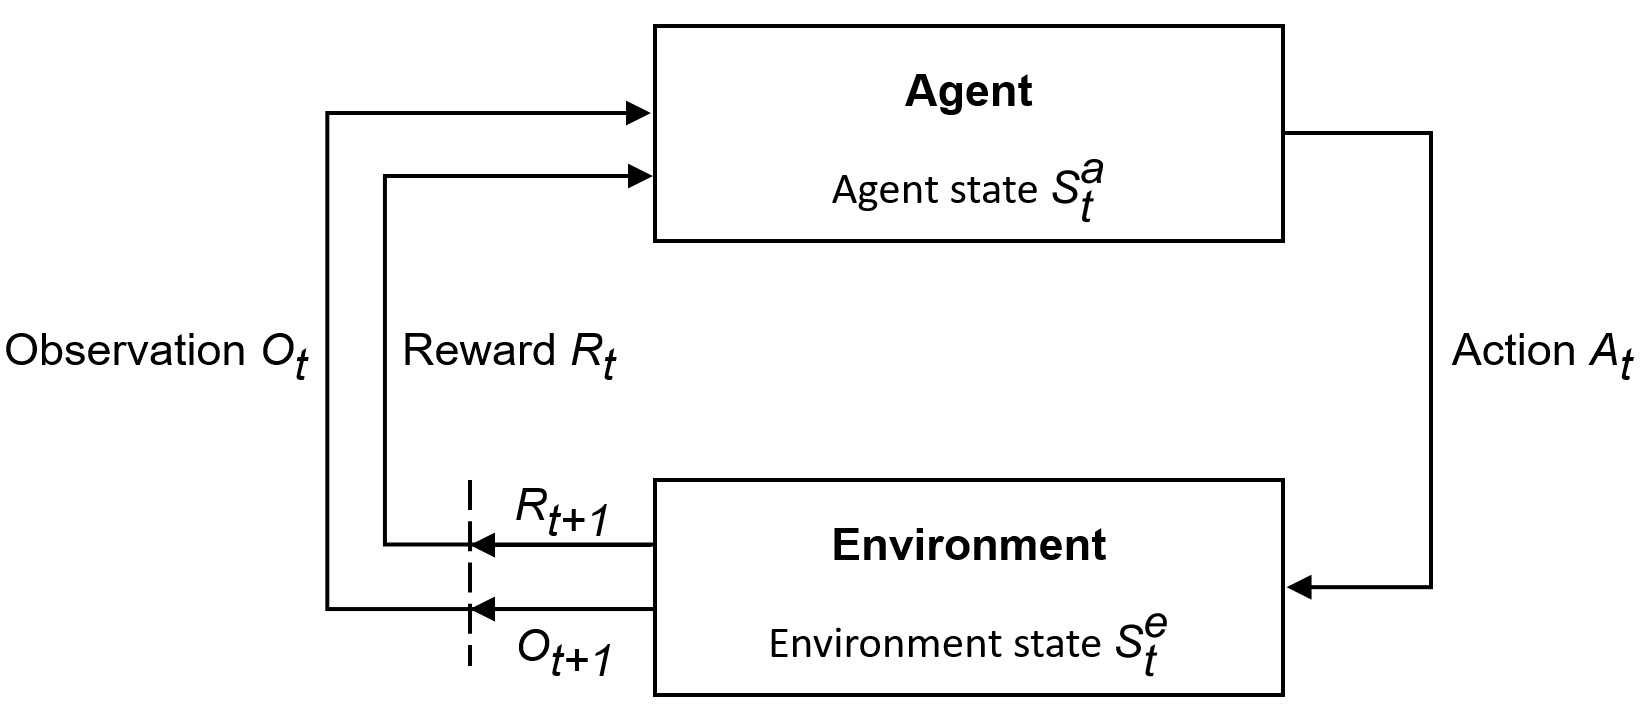
\includegraphics[height=5cm]{img/agent-env_POMDP.png}
\caption{POMDP framework (based on \textcite{silver2015})}
\label{fig:interaction-POMDP}
\end{figure}

\subsection{Policies}

The behaviour of an agent is defined by a policy $\pi$
\parencite{SuttonBarto_2018}. The policy is defined by the probability distribution of actions given the state (\autoref{equ:policy}). In other words, the policy determines which action the agent executes at each time step.

\begin{equation}
\label{equ:policy}
\pi(a|s) = Pr\lbrace A_t=a | S_t = s\rbrace
\end{equation}

%\subsection{On-Policy vs. Off-Policy Methods}

During the training of an \gls{rl} agent, there is a distinction between the behaviour policy and the target policy \parencite{Wang_2022}. The behaviour policy is the policy that the agent acts upon when generating training data. The target policy is the policy that is optimised through learning and should maximise the returns. 

With this distinction, \gls{rl} algorithms can be classified as either on-policy or off-policy \parencite{Wang_2022}. On-policy methods use the target policy as the behaviour policy. This means that in each round of optimisation, the target policy is used to generate the training samples. At the end of each round, these samples are discarded to avoid optimising on old policies.
In off-policy methods on the other hand, the target and behaviour policies differ. The samples are generated by the behaviour policies and are stored in a buffer. Samples from this buffer are then used to update the target policy.

Due to the fact that samples in the buffer can be re-used, off-policy methods have a higher data efficiency compared to on-policy methods \parencite{Wang_2022}. However, off-policy methods have more variance and converge slower than on-policy methods \parencite{SuttonBarto_2018}. 

\subsection{Value Functions}

The aim of an \gls{rl} agent is to maximise the total reward, which is also referred to as the return $G_t$ \parencite{SuttonBarto_2018}. This means that an agent should not only consider the immediate reward that is gained by taking an action, but future rewards should be considered as well. In \gls{rl}, the discounted return (\autoref{equ:disc_ret}) is usually considered. Here, the discount factor $\gamma \in [0, 1]$ weighs the importance of future rewards. If $\gamma = 0$, then the agent is only interested in the immediate rewards. As $\gamma$ increases, so does the importance of future rewards and the agent becomes increasingly far-sighted.

\begin{equation}
\label{equ:disc_ret}
G_t = R_{t+1} + \gamma R_{t+2} + \gamma^2 R_{t+3} + \gamma^3 R_{t+4} + ... = \sum^{\infty}_{k=0} \gamma^k R_{t+1+k}
\end{equation}

The expected return can be used to determine how good it is for an agent to be in a given state. This is quantified by the state-value-function $V(s)$, which gives the expected return when the agent starts in the state $s$ (\autoref{equ:state_val}). The higher the value, the better it is to be in the state. Using the Bellman equation, this can also be expressed in terms of the immediate reward and the discounted value of the next state (\autoref{equ:state_val_bellman}).

\begin{equation}
\label{equ:state_val}
V(s)= \mathbb{E}[G_t | S_t=s]
\end{equation}
\begin{equation}
\label{equ:state_val_bellman}
V(s)= \mathbb{E}[R_{t+1}+\gamma V(S_{t+1})| S_t=s]
\end{equation}

Likewise, the expected return can be used to determine how good an action is in a given state. The action-value function $Q(s, a)$ gives the expected return when the agent starts in the state $s$ and takes an action $a$ (\autoref{equ:action_val}). The higher the value, the better it is to take the action when in that state. This can also be transformed using the Bellman equation, which results in \autoref{equ:action_val_bellman}.

\begin{equation}
\label{equ:action_val}
Q(s, a)= \mathbb{E}[G_t | S_t=s, A_t=a]
\end{equation}
\begin{equation}
\label{equ:action_val_bellman}
Q(s, a)= \mathbb{E}[R_{t+1}+\gamma Q(S_{t+1}, A_{t+1}) | S_t=s, A_t=a]
\end{equation}

An optimal value function $V_*(s)$ or $Q_*(s, a)$ is defined as the value function that is obtained when following an optimal policy $\pi_*$ (Equations \ref{equ:optimal_state_val} and \ref{equ:optimal_action_val}). The optimal policy is the policy that maximises the return for all states.

\begin{equation}
\label{equ:optimal_state_val}
V_*(s)=\max_{\pi} V_\pi(s)
\end{equation}
\begin{equation}
\label{equ:optimal_action_val}
Q_*(s, a)=\max_{\pi} Q_\pi(s, a)
\end{equation}

\subsection{Reinforcement Learning Approaches}

One distinction that can be made when categorising \gls{rl} approaches is model-based vs. model-free \parencite{SuttonBarto_2018}. Model-based approaches require a model of the environment, which can be used to predict how the environment will behave. These models are used to evaluate potential next actions by considering all possible outcomes before they happen. This is referred to as planning.
% Examples for model-free algorithms are ...

Model-free approaches, on the other hand, learn through trial-and-error and do not require a model of the environment \parencite{SuttonBarto_2018}. Such approaches can be further classified as value-based methods, policy gradient methods or actor-critic methods.

Value-based algorithms aim to estimate the optimal value function \parencite{Wang_2022}. The optimal policy is implicitly given by the value function. For example, the target policy might be to behave greedily with respect to $Q_*(s, a)$. Examples for these algorithms are Q-Learning \parencite{Watkins_1992} and Deep Q-Learning (\gls{dqn}) \parencite{Mnih_2015}.

Policy gradient algorithms aim to optimise the target policy directly \parencite{Wang_2022}. Here, the parameterised policy $\pi_\theta(a|s)=Pr(a|s, \theta)$ is updated based on the gradient of a policy objective function $J(\theta)$. According to the policy gradient theorem, this can be calculated using \autoref{equ:policy-grad} \parencite{silver2015}. The benefit of this approach is that the policy does not become deterministic and therefore continues to allow for exploration \parencite{SuttonBarto_2018}. An example of a policy gradient algorithm is REINFORCE \parencite{Williams_1992}.

\begin{equation}
\label{equ:policy-grad}
\nabla_\theta J(\theta)=\mathbb{E}_{\pi_\theta}[Q_{\pi_\theta}(s, a)\cdot\nabla_\theta log\pi_\theta(a|s)]
\end{equation}

Actor-critic methods are methods that learn a policy and a value function at the same time \parencite{Wang_2022}. The actor generates policies, interacts with the environment and updates the target policy using the policy gradient. The critic learns the state-value function $V(s)$, action-value function $Q(s, a)$ or the advantage function $A(s, a)$ and uses this to evaluate the actor's policy. The advantage is defined in \autoref{equ:advantage} and represents the relative value of taking an action in a given state. This can be used instead of $Q(s, a)$ when calculating the gradient of the objective function (\autoref{equ:policy-grad}) to reduce the variance of the gradients.

\begin{equation}
\label{equ:advantage}
A(s, a)=Q(s, a)-V(s)
\end{equation}

%Value-Based methods: learn q values. Implicit policy is to select avtion with highest value. Doesnt require knowledge about environment. E.g. Q-learning (constructs table of q values, not scalable), DQN (uses function approximation to represent q-values usually NN).

%Policy-based methods: learn policy

%Actor-Critic methods:

%\begin{figure}[H]
%\centering
%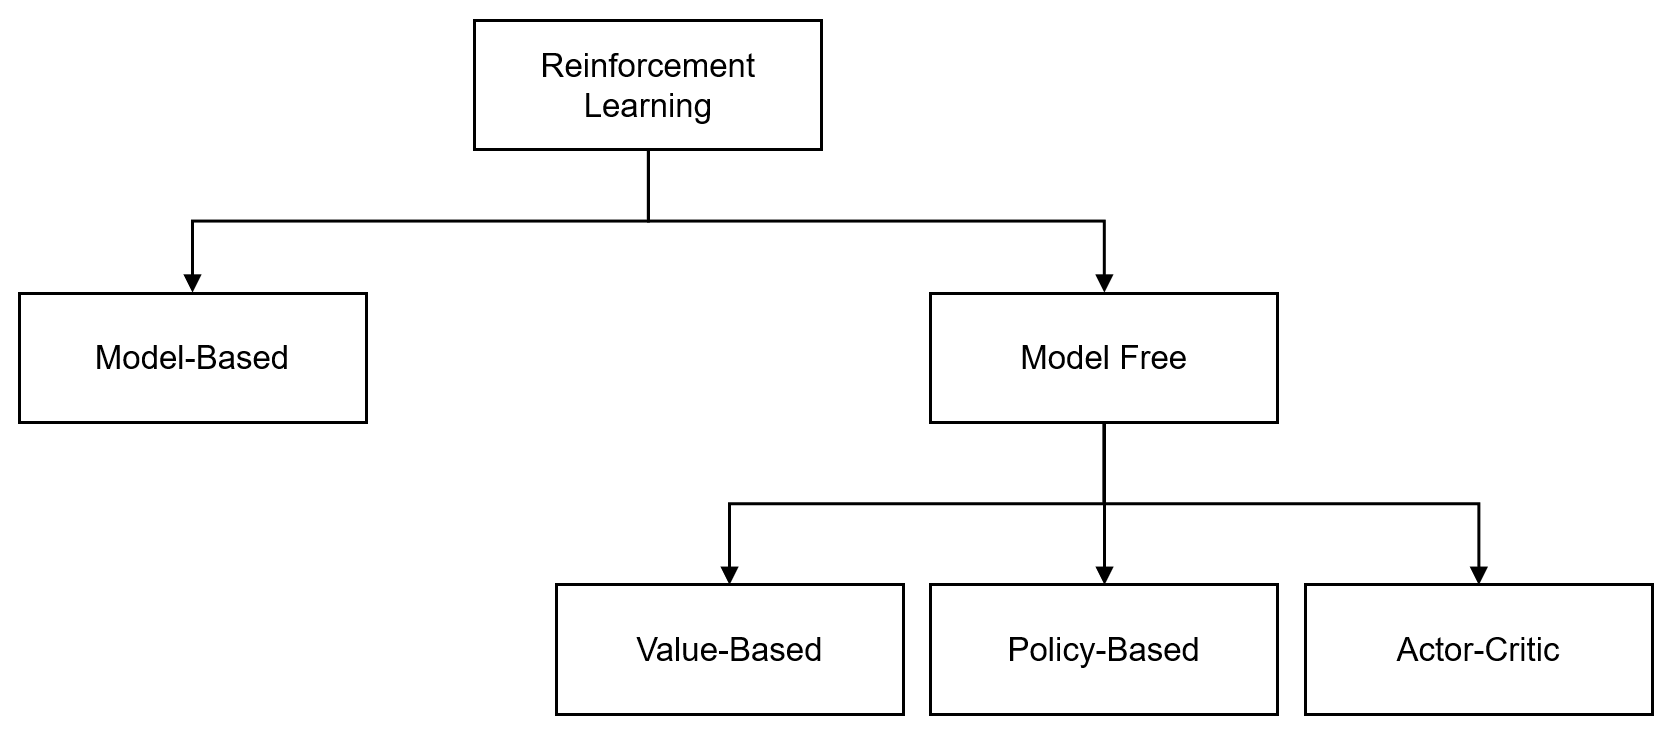
\includegraphics[height=5cm]{img/rl-approaches.png}
%\caption{Taxonomy of RL approaches}
%\label{fig:rl-approaches}
%\end{figure}






\section{Continual Learning}

Definition

\subsection{Continual Learning Problems}

Classification of problems

non-stationarity drivers etc.

\subsection{Continual Learning Agents}

ideal attributes of CL agent

CL Approaches

Explicit knowledge retention will be reviewed on more detail.

\subsection{Explicit Knowledge Retention}

\subsubsection{Latent Parameter Storage}

Definition

Discuss papers that do this

\subsubsection{Distillation Based}

Definition

Discuss papers that do this

\subsubsection{Rehearsal Based}

Definition

Discuss papers that do this


\section{Reinforcement Learning in Urban Traffic Control}
\chapter{Design}


\section{Proposed Algorithm}

Explain PPO and the approach to mitigate catastrophic forgetting

\section{Urban Traffic Control Environment}

Define environment

\section{Experiments}

Define the different experiments. Hypothesis?

Which baselines are used?

Re-run experiments with different seeds to so statistical evaluations
\chapter{Implementation}

Tools used etc.
\chapter{Evaluation}

\section{Experimental Results}
Present results and discuss them

\section{Future Work}

Improvements that could be done in the future
\chapter{Conclusion}

Summary

\addcontentsline{toc}{chapter}{References}
\printbibliography[title={References}]

\appendix

\end{document}